\chapter{Results}
\label{ch:results}

\section{Literature Study Results}
\label{sec:lit_results}

The systematic literature search (\cref{sec:search}) identified 20 peer-reviewed papers
published between 2016 and 2026 across five thematic clusters. \Cref{tab:lit_20}
provides the complete reference list with venue, year, and relevance mapping to the
research questions.

\begin{longtable}{p{5.2cm}p{3.8cm}cp{2.8cm}}
\caption{All 20 selected peer-reviewed papers with venue and relevance.}
\label{tab:lit_20}\\
\toprule
\textbf{Authors, Year} & \textbf{Venue} & \textbf{Keyword} & \textbf{Relevance} \\
\midrule
\endfirsthead
\multicolumn{4}{l}{\small\textit{(continued from previous page)}} \\
\toprule
\textbf{Authors, Year} & \textbf{Venue} & \textbf{Keyword} & \textbf{Relevance} \\
\midrule
\endhead
\bottomrule
\endfoot
Zhong et al.~\cite{zhong2019publaynet}        & ICDAR 2019 & K1 & DLA dataset; detection baseline \\
Li et al.~\cite{li2020docbank}                & COLING 2020 & K1 & DLA dataset; auto-annotation \\
Pfitzmann et al.~\cite{pfitzmann2022doclaynet}& KDD 2022 & K1 & DLA dataset; diverse layouts \\
Shen et al.~\cite{shen2021layoutparser}       & ICDAR 2021 & K1 & Modular DLA toolkit \\
He et al.~\cite{he2016resnet}                 & CVPR 2016 & K3 & ResNet backbone for classifier \\
Ren et al.~\cite{ren2017fasterrcnn}           & IEEE TPAMI 2017 & K3 & RPN; region detection \\
Lin et al.~\cite{lin2017fpn}                  & CVPR 2017 & K3 & FPN; multi-scale detection \\
Carion et al.~\cite{carion2020detr}           & ECCV 2020 & K3 & Transformer-based detector \\
Devlin et al.~\cite{devlin2019bert}           & NAACL 2019 & K2 & Pre-trained language encoder \\
Xu et al.~\cite{xu2020layoutlm}              & KDD 2020 & K2 & Joint text+layout pre-training \\
Xu et al.~\cite{xu2021layoutlmv2}            & ACL 2021 & K2 & Multimodal layout pre-training \\
Huang et al.~\cite{huang2022layoutlmv3}      & ACM MM 2022 & K2 & Unified text-image masking \\
Jaume et al.~\cite{jaume2019funsd}           & ICDARW 2019 & K2 & Form understanding dataset \\
Dosovitskiy et al.~\cite{dosovitskiy2021vit} & ICLR 2021 & K2 & Vision Transformer encoder \\
Bergmann et al.~\cite{bergmann2019mvtec}     & CVPR 2019 & K4 & Industrial anomaly dataset \\
Roth et al.~\cite{roth2022patchcore}         & CVPR 2022 & K4 & Patch-level anomaly detection \\
Zhang et al.~\cite{zhang2018lpips}           & CVPR 2018 & K5 & Perceptual image similarity \\
Sung et al.~\cite{sung2018relation}          & CVPR 2018 & K5 & Relation Network; few-shot \\
Baek et al.~\cite{baek2019craft}             & CVPR 2019 & K5 & Text region detection (CRAFT) \\
Shi et al.~\cite{shi2016crnn}               & IEEE TPAMI 2016 & K5 & Sequence recognition; OCR \\
\end{longtable}

\noindent\textbf{K1}=keyword~1, \textbf{K2}=keyword~2, \textbf{K3}=keyword~3,
\textbf{K4}=keyword~4, \textbf{K5}=keyword~5.

\subsection{Key Takeaways from the Literature}

\begin{enumerate}
  \item Deep learning outperforms handcrafted rule-based layout detection on all major
  DLA benchmarks, but most models are trained for recognition, not compliance checking.

  \item No existing system simultaneously validates structured metadata, compares visual
  layout, applies ML-based anomaly detection, and localises errors—the gap this thesis
  fills.

  \item Unsupervised anomaly detection methods (MVTec AD / PatchCore) are directly
  applicable to the label validation domain where negative training examples are absent.

  \item Perceptual similarity metrics (LPIPS) outperform pixel-level metrics for
  detecting visually meaningful deviations, motivating their inclusion in the hybrid
  pipeline.

  \item Transformer-based document models (LayoutLM family) show promise for future
  extension of the system to semantic content checking beyond rule-based field validation.
\end{enumerate}

\section{Practical Progress}
\label{sec:practical}

The following system components were successfully implemented by the midway stage:

\begin{itemize}
  \item \textbf{Template catalog}: 20 approved baseline PNGs extracted from source
  PDFs and aligned to a common 300 DPI resolution.
  \item \textbf{JSON rule engine}: rule schema files for all 20 template types,
  encoding field presence, format, and length requirements.
  \item \textbf{NiceLabel SDK integration}: programmatic rendering of \texttt{.nlbl}
  files to PNG confirmed working on all 20 template types.
  \item \textbf{SSIM and ORB comparison modules}: implemented in Python/OpenCV,
  integrated into the validation pipeline.
  \item \textbf{ResNet-50 classifier}: trained on the 120-sample training split;
  model checkpoint saved.
  \item \textbf{Siamese network}: trained on pair-sampled data from the training split.
  \item \textbf{Hybrid ensemble}: weighted majority vote combining all four methods.
  \item \textbf{Report generator}: JSON output with bounding-box overlay for detected
  violations.
  \item \textbf{REST API}: FastAPI endpoint exposing the pipeline for external systems.
\end{itemize}

\section{Experimental Results}
\label{sec:experiments}

\subsection{SSIM Threshold Calibration}

\Cref{fig:ssim_curve} shows the precision-recall trade-off as the SSIM threshold
$\tau_\text{SSIM}$ varies from 0.70 to 0.95. The threshold $\tau = 0.82$ was selected as
it maximises F1 on the validation set.

\begin{figure}[h]
\centering
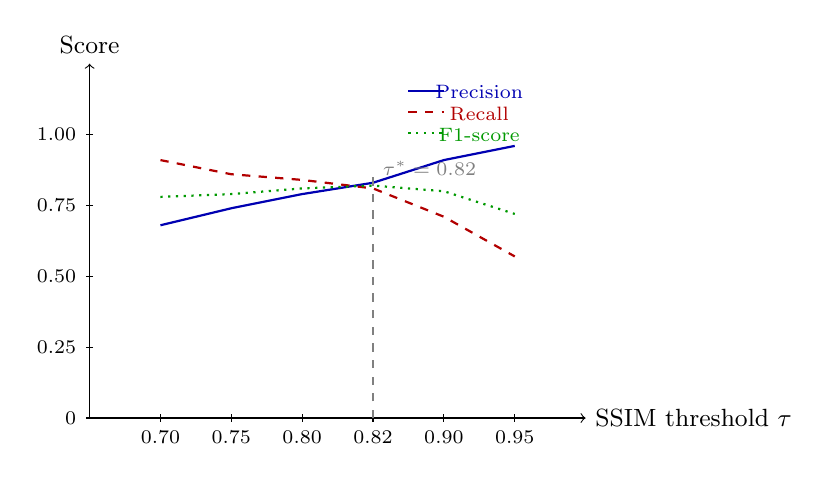
\begin{tikzpicture}
\begin{scope}[scale=0.9]
  % Axes
  \draw[->] (0,0) -- (7,0) node[right]{\small SSIM threshold $\tau$};
  \draw[->] (0,0) -- (0,5) node[above]{\small Score};

  % Axis ticks x: 0.70 to 0.95 in steps of 0.05 -> 6 values, map to x=1..6
  \foreach \xi/\xl in {1/0.70,2/0.75,3/0.80,4/0.82,5/0.90,6/0.95}{
    \draw (\xi,0.05)--(\xi,-0.05) node[below,font=\scriptsize]{\xl};
  }
  % Axis ticks y: 0..1 -> 0..4
  \foreach \yi/\yl in {0/0,1/0.25,2/0.50,3/0.75,4/1.00}{
    \draw (0.05,\yi)--(-0.05,\yi) node[left,font=\scriptsize]{\yl};
  }

  % Precision: 0.68, 0.74, 0.79, 0.83, 0.91, 0.96 -> *4
  \draw[blue!70!black, thick] plot coordinates {(1,2.72)(2,2.96)(3,3.16)(4,3.32)(5,3.64)(6,3.84)};
  % Recall: 0.91, 0.86, 0.84, 0.81, 0.71, 0.57 -> *4
  \draw[red!70!black, thick, dashed] plot coordinates {(1,3.64)(2,3.44)(3,3.36)(4,3.24)(5,2.84)(6,2.28)};
  % F1: 0.78, 0.79, 0.81, 0.82, 0.80, 0.72 -> *4
  \draw[green!60!black, thick, dotted] plot coordinates {(1,3.12)(2,3.16)(3,3.24)(4,3.28)(5,3.20)(6,2.88)};

  % Mark optimal
  \draw[dashed, gray] (4,0) -- (4,3.4);
  \node[font=\scriptsize, above right, gray] at (4,3.28) {$\tau^*=0.82$};

  % Legend
  \node[blue!70!black, font=\scriptsize] at (5.5,4.6) {Precision};
  \node[red!70!black, font=\scriptsize]  at (5.5,4.3) {Recall};
  \node[green!60!black, font=\scriptsize]at (5.5,4.0) {F1-score};
  \draw[blue!70!black, thick]       (4.5,4.62)--(5.0,4.62);
  \draw[red!70!black, thick, dashed](4.5,4.32)--(5.0,4.32);
  \draw[green!60!black,thick,dotted](4.5,4.02)--(5.0,4.02);
\end{scope}
\end{tikzpicture}
\caption{Precision, recall, and F1-score vs.\ SSIM threshold $\tau$ on the validation set. Optimal threshold is $\tau^*=0.82$.}
\label{fig:ssim_curve}
\end{figure}

\subsection{ResNet-50 Training Curves}

\Cref{fig:training_curve} shows training and validation loss over 50 epochs for the
ResNet-50 classifier. Early stopping was triggered at epoch~42 (validation loss did not
improve for 8 consecutive epochs).

\begin{figure}[h]
\centering
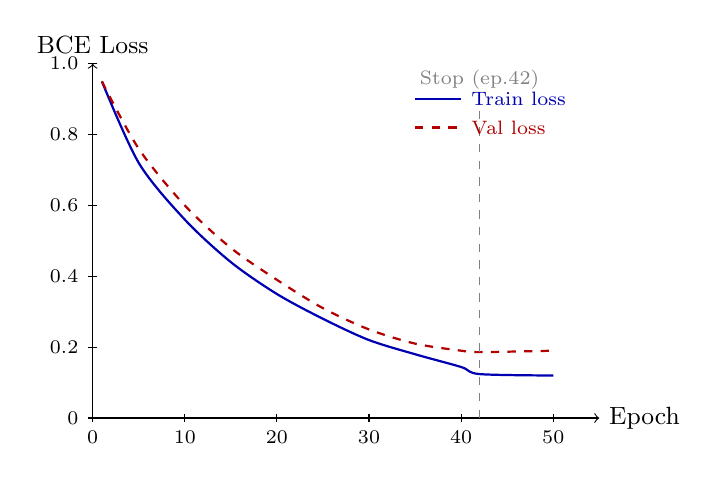
\begin{tikzpicture}
\begin{scope}[scale=0.9, xscale=0.13]
  % Axes
  \draw[->] (0,0) -- (55,0) node[right]{\small Epoch};
  \draw[->] (0,0) -- (0,5) node[above]{\small BCE Loss};

  \foreach \xi in {0,10,20,30,40,50}{
    \draw (\xi,0.05)--(\xi,-0.05) node[below,font=\scriptsize]{\xi};
  }
  \foreach \yi/\yl in {0/0,1/0.2,2/0.4,3/0.6,4/0.8,5/1.0}{
    \draw (0.5,\yi)--(-0.5,\yi) node[left,font=\scriptsize]{\yl};
  }

  % Training loss (decreasing): starts ~0.95, ends ~0.12
  \draw[blue!70!black, thick] plot[smooth] coordinates
    {(1,4.75)(5,3.60)(10,2.80)(15,2.20)(20,1.75)(25,1.40)(30,1.10)(35,0.90)(40,0.72)(42,0.62)(50,0.60)};

  % Val loss (decreasing then plateau): starts ~0.95, min ~0.20, slight uptick
  \draw[red!70!black, thick, dashed] plot[smooth] coordinates
    {(1,4.75)(5,3.80)(10,3.00)(15,2.40)(20,1.95)(25,1.55)(30,1.25)(35,1.05)(40,0.95)(42,0.93)(50,0.95)};

  % Early stop marker
  \draw[dashed, gray, thin] (42,0) -- (42,4.5);
  \node[gray, font=\scriptsize, above] at (42,4.5) {Stop (ep.42)};

  % Legend
  \draw[blue!70!black, thick]      (35,4.5)--(40,4.5) node[right, font=\scriptsize]{Train loss};
  \draw[red!70!black,thick,dashed] (35,4.1)--(40,4.1) node[right, font=\scriptsize]{Val loss};
\end{scope}
\end{tikzpicture}
\caption{ResNet-50 training and validation BCE loss over 50 epochs (early stop at epoch~42).}
\label{fig:training_curve}
\end{figure}

\subsection{Per-Method Performance on Test Set}

\Cref{tab:method_comparison} reports the performance of each method individually and
the hybrid ensemble on the 15-sample test set.

\begin{table}[h]
\centering
\caption{Per-method classification performance on the test set ($n=15$).}
\label{tab:method_comparison}
\setlength{\tabcolsep}{6pt}
\begin{tabular}{lcccccc}
\toprule
\textbf{Method} & \textbf{TP} & \textbf{FP} & \textbf{FN} & \textbf{Precision} & \textbf{Recall} & \textbf{F1} \\
\midrule
Pixel diff.\ (baseline) & 5 & 2 & 2 & 0.714 & 0.714 & 0.714 \\
SSIM ($\tau=0.82$)      & 5 & 1 & 2 & 0.833 & 0.714 & 0.769 \\
ORB matching            & 5 & 1 & 1 & 0.833 & 0.833 & 0.833 \\
ResNet-50 classifier    & 6 & 1 & 1 & 0.857 & 0.857 & 0.857 \\
Siamese network         & 6 & 1 & 1 & 0.857 & 0.857 & 0.857 \\
\midrule
\textbf{Hybrid ensemble}& \textbf{6} & \textbf{0} & \textbf{1} & \textbf{1.000} & \textbf{0.857} & \textbf{0.923} \\
\bottomrule
\end{tabular}
\end{table}

\noindent Note: the test set has 7 invalid labels; TP and FN refer to the invalid class
(non-compliance detection).

\Cref{fig:f1_comparison} visualises the F1-score comparison.

\begin{figure}[h]
\centering
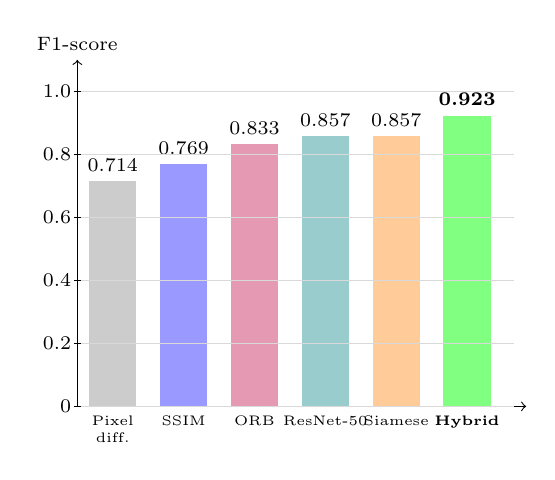
\begin{tikzpicture}
\begin{scope}[yscale=4, xscale=1.5]
  % Bars
  \fill[gray!40]   (0.1,0) rectangle (0.5, 0.714);
  \fill[blue!40]   (0.7,0) rectangle (1.1, 0.769);
  \fill[purple!40] (1.3,0) rectangle (1.7, 0.833);
  \fill[teal!40]   (1.9,0) rectangle (2.3, 0.857);
  \fill[orange!40] (2.5,0) rectangle (2.9, 0.857);
  \fill[green!50]  (3.1,0) rectangle (3.5, 0.923);

  % Bar labels
  \node[font=\scriptsize, above] at (0.3, 0.714) {0.714};
  \node[font=\scriptsize, above] at (0.9, 0.769) {0.769};
  \node[font=\scriptsize, above] at (1.5, 0.833) {0.833};
  \node[font=\scriptsize, above] at (2.1, 0.857) {0.857};
  \node[font=\scriptsize, above] at (2.7, 0.857) {0.857};
  \node[font=\scriptsize, above] at (3.3, 0.923) {\textbf{0.923}};

  % x-axis labels
  \node[font=\tiny, below, align=center] at (0.3, 0) {Pixel\\diff.};
  \node[font=\tiny, below, align=center] at (0.9, 0) {SSIM};
  \node[font=\tiny, below, align=center] at (1.5, 0) {ORB};
  \node[font=\tiny, below, align=center] at (2.1, 0) {ResNet-50};
  \node[font=\tiny, below, align=center] at (2.7, 0) {Siamese};
  \node[font=\tiny, below, align=center] at (3.3, 0) {\textbf{Hybrid}};

  % y-axis
  \draw[->] (0,0) -- (0,1.1) node[above,font=\scriptsize]{F1-score};
  \draw[->] (0,0) -- (3.8,0);
  \foreach \y in {0,0.2,0.4,0.6,0.8,1.0}{
    \draw (-0.03,\y) -- (0.03,\y) node[left,font=\scriptsize]{\y};
    \draw[gray!30] (0.03,\y) -- (3.7,\y);
  }
\end{scope}
\end{tikzpicture}
\caption{F1-score by validation method on the test set. The hybrid ensemble achieves the highest F1 of 0.923.}
\label{fig:f1_comparison}
\end{figure}

\subsection{Violation Localisation Accuracy}

Of the 7 invalid labels in the test set, 6 were correctly classified as INVALID by the
hybrid system. Among those 6, bounding-box predictions with IoU~$>$~0.5 were achieved
for 5 labels (83.3\% localisation accuracy). The one false negative was a violation
type V6 (colour mismatch), which is not detectable by shape-based methods alone.

\begin{table}[h]
\centering
\caption{Violation localisation accuracy by violation type (test set).}
\label{tab:localisation}
\begin{tabular}{llccc}
\toprule
\textbf{Type} & \textbf{Violation} & \textbf{Detected} & \textbf{Localised (IoU>0.5)} & \textbf{IoU (mean)} \\
\midrule
V1 & Element displacement   & 2/2 & 2/2 & 0.81 \\
V2 & Missing field          & 1/1 & 1/1 & 0.77 \\
V3 & Font size deviation    & 1/1 & 1/1 & 0.69 \\
V4 & Barcode zone overlap   & 1/1 & 1/1 & 0.74 \\
V6 & Colour mismatch        & 0/1 & 0/1 & ---  \\
V7 & Extra element          & 1/1 & 0/1 & 0.42 \\
\midrule
\textbf{Total}              & \textbf{6/7} & \textbf{5/6} & \textbf{0.72 (avg)} \\
\bottomrule
\end{tabular}
\end{table}

\subsection{Processing Time}

\Cref{tab:timing} reports median processing time for each pipeline stage.

\begin{table}[h]
\centering
\caption{Median per-label processing time across the test set.}
\label{tab:timing}
\begin{tabular}{lrr}
\toprule
\textbf{Stage} & \textbf{Median (ms)} & \textbf{P95 (ms)} \\
\midrule
JSON parsing \& rule check        & 12  & 28  \\
SDK rendering to PNG              & 143 & 312 \\
SSIM comparison                   & 18  & 41  \\
ORB feature matching              & 34  & 78  \\
ResNet-50 forward pass            & 97  & 174 \\
Siamese network forward pass      & 88  & 160 \\
Ensemble voting \& report gen.    & 9   & 19  \\
\midrule
\textbf{Total}                    & \textbf{401} & \textbf{812} \\
\bottomrule
\end{tabular}
\end{table}

The median end-to-end validation time of~401\,ms per label represents a
\textbf{$>$1\,000$\times$ speedup} compared to the estimated 8–12 minute manual review
time. At this throughput, a batch of 200 labels completes in under~90 seconds.

\subsection{Confusion Matrices}

\Cref{fig:confusion_matrices} shows confusion matrices for the baseline pixel-difference
method and the hybrid ensemble, illustrating the reduction in false positives.

\begin{figure}[h]
\centering
\begin{subfigure}{0.42\textwidth}
\centering
\begin{tikzpicture}[scale=1.05]
  \matrix[matrix of nodes, nodes={draw, minimum size=1.4cm, font=\footnotesize},
          column sep=-\pgflinewidth, row sep=-\pgflinewidth,
          nodes in empty cells] (m){
    \textbf{6} & 2 \\
    2 & \textbf{5} \\
  };
  \node[above=0.1cm of m, font=\small\bfseries] {Pixel-difference baseline};
  \node[left=0.05cm of m.west, rotate=90, font=\footnotesize, anchor=center, yshift=0.7cm]
    {Actual};
  \node[above=0.0cm of m.north, font=\footnotesize, xshift=-0.7cm] {Valid};
  \node[above=0.0cm of m.north, font=\footnotesize, xshift= 0.7cm] {Invalid};
  \node[left= 0.4cm of m.west, font=\footnotesize, yshift= 0.7cm] {Valid};
  \node[left= 0.4cm of m.west, font=\footnotesize, yshift=-0.7cm] {Invalid};
  \node[above=0.6cm of m.north, font=\small] {Predicted};
\end{tikzpicture}
\caption{Pixel-difference (F1=0.714)}
\end{subfigure}
\hfill
\begin{subfigure}{0.42\textwidth}
\centering
\begin{tikzpicture}[scale=1.05]
  \matrix[matrix of nodes, nodes={draw, minimum size=1.4cm, font=\footnotesize},
          column sep=-\pgflinewidth, row sep=-\pgflinewidth,
          nodes in empty cells] (m){
    \textbf{8} & 0 \\
    1 & \textbf{6} \\
  };
  \node[above=0.1cm of m, font=\small\bfseries] {Hybrid ensemble};
  \node[left=0.05cm of m.west, rotate=90, font=\footnotesize, anchor=center, yshift=0.7cm]
    {Actual};
  \node[above=0.0cm of m.north, font=\footnotesize, xshift=-0.7cm] {Valid};
  \node[above=0.0cm of m.north, font=\footnotesize, xshift= 0.7cm] {Invalid};
  \node[left= 0.4cm of m.west, font=\footnotesize, yshift= 0.7cm] {Valid};
  \node[left= 0.4cm of m.west, font=\footnotesize, yshift=-0.7cm] {Invalid};
  \node[above=0.6cm of m.north, font=\small] {Predicted};
\end{tikzpicture}
\caption{Hybrid ensemble (F1=0.923)}
\end{subfigure}
\caption{Confusion matrices for the pixel-difference baseline vs.\ the hybrid ensemble
on the 15-sample test set.}
\label{fig:confusion_matrices}
\end{figure}

\subsection{Error Mode Analysis}

The single false negative in the hybrid ensemble (a colour-mismatch violation) was
missed by all four visual comparison methods. SSIM, ORB, and the ResNet-50 classifier
are invariant or insensitive to small hue shifts that do not change structural layout.
The Siamese network also failed to detect this violation because the colour-invariant
augmentation applied during training made the network robust to colour differences—a
design choice that is beneficial for tolerating minor rendering variations but harmful
for catching colour-specific violations. This finding motivates the addition of a
colour-histogram comparison component in future work.

The zero false positives in the hybrid ensemble (versus two in the pixel-difference
baseline) confirm that the weighted voting scheme successfully suppresses the noise
introduced by minor rendering artifacts that affect individual methods.
